\documentclass{article}

\usepackage{hyperref}          % Clickable link
\usepackage{indentfirst}

% References
\usepackage{biblatex}
\addbibresource{references.bib}
\usepackage[final]{microtype}

% Images
\usepackage{graphicx}          % Load images
\usepackage{float}             % Insert images at the current position using [h]
\graphicspath{ {./images/} }
\usepackage{wrapfig}     % Text wrap image

% SVG
\usepackage{ifluatex}
\ifluatex
  \usepackage{pdftexcmds}
  \makeatletter
  \let\pdfstrcmp\pdf@strcmp
  \let\pdffilemoddate\pdf@filemoddate
  \makeatother
\fi
\usepackage{svg}

% Change names of document elements
\renewcommand{\figurename}{Hình}

\usepackage{textcomp}    % For the Trade Mark joke


\author{Nguyễn Việt Minh Nghĩa \\ \href{mailto:nvmnghia@gmail.com}{nvmnghia@gmail.com}}

\date{11/04/2020}

\title{Kiến trúc hướng dịch vụ INT3505 \\ Bài tập lớn số hai \\ Tìm hiểu về Message-oriented Middleware}

\begin{document}

\maketitle

\section{Giới thiệu}

\subsection{Tiền đề}

Với sự phát triển của công nghiệp bán dẫn, máy tính ngày nay trở nên nhanh hơn,
phổ biến hơn. Tuy nhiên, do hạn chế về vật lý, việc tăng tốc phần cứng của một
hệ thống phần mềm không thể chỉ thực hiện được bằng cách làm ra một máy tính lớn
hơn, mạnh hơn (scale up), mà còn phải bằng cách tăng số lượng các máy (scale
out).

Song song với phần cứng, phần mềm cũng trở nên phức tạp hơn. Một hệ thống phần
mềm ngày nay gồm nhiều hệ thống con có mức chuyên biệt hóa cao hoạt động độc
lập, thay vì một khối phần mềm lớn (monolithic) như trước. Cho dù các thành phần
của hệ thống này cùng chạy trên một máy, chúng cũng không thể đơn giản là dùng
chung một khối bộ nhớ, do cơ chế bảo mật địa chỉ ảo của hệ điều hành.

Hai vấn đề này cùng dẫn đến nhu cầu kết nối các máy tính (hay cụ thể hơn, các
tiến trình) với nhau, và trao đổi dữ liệu giữa chúng. Với sự phát triển của mạng
máy tính tốc độ cao, các giải pháp kết nối máy tính bắt đầu có thể thực hiện
được. Xét về mặt phần mềm, các cơ chế để giải quyết vấn đề này được gọi là giao
tiếp liên tiến trình, thường gọi là IPC (viết tắt của inter-process
communication).

\subsection{Giao tiếp liên tiến trình - IPC}

Có rất nhiều cơ chế để liên lạc giữa các tiến trình với nhau, nổi bật trong số
đó có RPC - Remote Procedure Call. Hai trong những lí do cho sự phổ biến của RPC
là nó có thể giúp cho các tiến trình ở các máy khác nhau giao tiếp được với
nhau, đồng thời không phụ thuộc vào ngôn ngữ. Nhiều phương pháp cũ hơn như file,
pipe, shared memory, ... đều không thể thực hiện việc này \cite{osc12}. Tuy
nhiên, RPC và các biến thể của nó như ORB rất khó đáp ứng với các yêu cầu mới về
độ ổn định, khả năng hoạt động liên tục và hiệu năng, khiến nó dần trở nên lỗi
thời.

Để giải quyết các hạn chế của RPC, có một cơ chế mới đang được sử dụng rất nhiều
hiện nay là Message-oriented Middleware, viết tắt là MOM.

\subsection{Message-oriented Middleware}

MOM là một lớp trung gian giúp gửi và nhận dữ liệu \emph{theo kiểu thông điệp}
(message-passing) giữa hai tiến trình khác nhau. Các danh từ khác thường được
coi là đồng nghĩa với MOM là hàng đợi thông điệp (message queue), hay trung gian
chuyển thông điệp (message broker).

Thông thường, một hệ thống MOM có ba thành phần:

\begin{itemize}
    \item Producer: Nguồn gửi thông điệp
    \item Broker: Trung gian trung chuyển thông điệp
    \item Consumer: Điểm nhận thông điệp
\end{itemize}

Ý tưởng trung tâm của MOM là giao tiếp bằng \emph{thông điệp}. Thông tin được
gửi ở dạng thông điệp, giống như tin nhắn hay gửi thư, thay thế cho việc
producer phải chủ động liên lạc trực tiếp với consumer. Nói cách khác, producer
được \emph{giải phóng khỏi việc gửi thông tin}.

Hình \ref{general_producer_broker_consumer} mô tả kiến trúc của một MOM đơn
giản, với ba thành phần kể trên (mũi tên chỉ hướng đi của thông điệp):

% graph TD
%   p1[Producer 1] --> b(Broker)
%   p2[Producer 2] --> b(Broker)
%   p3[Producer 3] --> b(Broker)

%   b(Broker) --> c1[Consumer 1]
%   b(Broker) --> c2[Consumer 2]

\begin{figure}[H]
    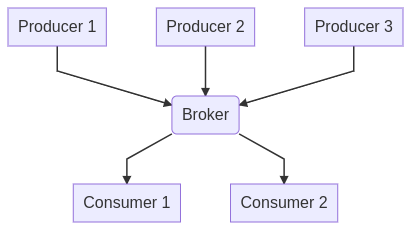
\includegraphics[scale=0.5]{general_producer_broker_consumer.png}
    \centering
    \caption{Kiến trúc chung của MOM.}
    \label{general_producer_broker_consumer}
\end{figure}

Bài này sẽ phân tích các đặc điểm và kiến trúc cơ bản của một hệ thống MOM, đồng
thời giới thiệu về Apache Kafka, một trong các MOM được sử dụng nhiều nhất hiện
nay.

\section{Đặc điểm}

Để tìm hiểu đặc điểm của MOM, ta có thể so sánh MOM với một cơ chế IPC khác
có khả năng gần giống là RPC.

\subsection{Tính bất đồng bộ - Asynchrony}

Tính bất đồng bộ là đặc điểm quan trọng nhất của ý tưởng giao tiếp thông qua
thông điệp \cite{inbook}. Thuộc tính này nghĩa là producer chỉ cần "gửi" một
thông điệp, thông điệp đó sẽ được broker đưa đến consumer phù hợp để xử lí. Để
thấy rõ lợi ích của tính bất đồng bộ, ta có thể so sánh với RPC đồng bộ (có RPC
bất đồng bộ, nhưng ta tạm thời bỏ qua).

Với RPC, khi client gọi một hàm của server, dữ liệu (ở dạng các tham số đầu vào)
được marshall và gửi sang server. Sau khi server xử lí xong, dữ liệu (kết quả
đầu ra) lại được gửi lại client. Trong suốt thời gian gửi-xử lí-nhận đó, client
phải chờ (blocking), gây ra chậm trễ đáng kể và lãng phí thời gian. Nếu có vấn
đề về mạng, hoặc một lí do nào khác không thể gửi/nhận dữ liệu, client phải gửi
lại.

Với MOM, khi producer gọi muốn gửi dữ liệu sang consumer, producer chỉ cần giao
dữ liệu cho broker, và broker sẽ tự gửi đến consumer. Ngay sau đó, producer có
thể làm việc khác, không phí thời gian chờ kết quả. Nếu ngay lúc đó consumer
không thể nhận được dữ liệu, broker sẽ chờ đến khi consumer có thể nhận được dữ
liệu rồi gửi lại, đảm bảo gửi ít nhất một lần.

Cần chú ý rằng MOM không thể, và không được thiết kế để thay thế hoàn toàn RPC.
Lý do chính nằm ở chi tiết producer không chờ lấy dữ liệu kết quả. MOM hoàn toàn
không cung cấp một cơ chế riêng nào giúp consumer trả kết quả cho producer, trái
ngược với tính liên lạc hai chiều của RPC. Nếu muốn lấy kết quả, hai bên
producer và consumer đổi vai cho nhau, và cần thêm một kết nối nữa. Điều này
khiến cho RPC vẫn có chỗ đứng riêng, đồng thời khiến cho việc thiết kế hệ thống
dùng MOM có khác biệt lớn so với với hệ thống dùng RPC: MOM chỉ phù hợp với hệ
thống có dữ liệu không có sự phụ thuộc lẫn nhau \cite{ejb3_c4}.

\subsection{Tách rời bên gửi - bên nhận - Decoupling}

Một đặc điểm quan trọng khi tách việc "gửi" dữ liệu khỏi producer là việc gửi đi
đâu hoàn toàn nằm trong tay broker. Động từ "gửi" được dùng theo nghĩa là một
bên muốn bên kia biết được một thông tin nào đó. Để có thể gửi, bên gửi cần biết
thông tin bên nhận. Tuy nhiên, với MOM, bên "gửi" - producer - có thể không cần
biết thông tin của bên "nhận" - consumer. Producer không cần biết rằng consumer
nào nhận, chứ chưa nói đến việc có bao nhiêu consumer nhận, hay đã nhận được
thực sự chưa.

Nói đơn giản, với producer và ngưòi dùng, MOM là một dịch vụ gửi thông điệp theo
kiểu bắn-và-quên. Hệ thống MOM do đó đạt được sự tách rời gửi-nhận.

Tiếp tục so sánh với RPC, bên gửi cần biết thông tin về bên nhận (ví dụ như địa
chỉ IP, tên hàm, ...). Nếu có nhiều bên nhận, bên gửi phải xử lí việc gửi cho
mọi bên nhận, bao gồm những việc như chờ, gửi lại nếu bị lỗi, ..., do đó tốn
nhiều thời gian. Đặc biệt, với các hệ thống đám mây, nơi việc máy chủ ảo bị xóa,
tắt, hoặc tạo mới diễn ra thường xuyên thì mạng kết nối đầy đủ, chặt chẽ (fully
connected network) mà RPC tạo ra sẽ rất phức tạp và khó bảo trì
\cite{Kleppmann17C}, giống như biếm họa trong hình
\ref{spaghetti_architectures}.

\begin{figure}[H]
    \centering
    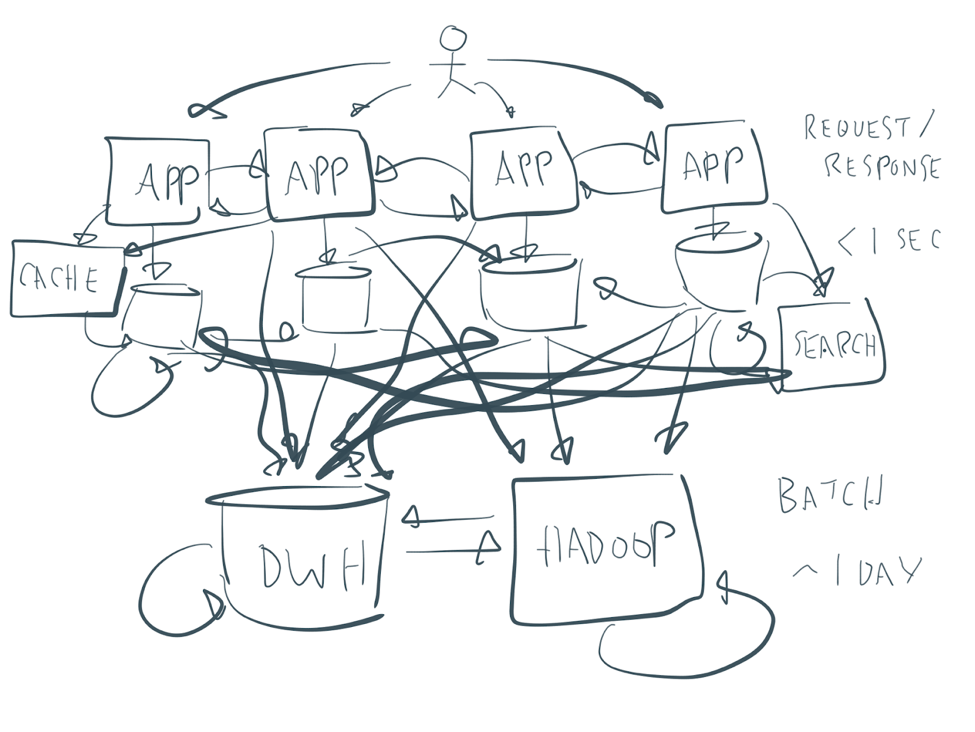
\includegraphics[scale=0.5]{spaghetti_architectures.png}
    \caption{Kiến trúc Spaghetti\texttrademark \cite{confluent2018}.}
    \label{spaghetti_architectures}
\end{figure}

Với hai đặc điểm nêu trên, có thể thấy rằng hệ thống sử dụng MOM có thiết kế
hoàn toàn khác với hệ thống sử dụng RPC:

\begin{itemize}
    \item MOM phù hợp với hệ thống được thiết kế có liên kết lỏng lẻo
    (loose-coupling).
    \item RPC phù hợp với hệ thống cần liên lạc hai chiều.
\end{itemize}

\section{Trung gian trung chuyển thông điệp - Message broker}

Trung gian trung chuyển thông điệp là thành phần chính trong một hệ thống MOM,
chịu trách nhiệm trung chuyển dữ liệu. Dù broker được coi là một thành phần
trong bản thân MOM, nó là thành phần chính yếu nhất, và trong nhiều trường hợp
cụm từ "message broker" được sử dụng tương đương với cụm từ MOM. Do vậy, ta có
thể tạm bỏ qua producer và consumer, và phân tích broker.

Trưóc đây, các hệ thống broker thường chỉ được dùng trong các hệ thống của tổ
chức lớn, do tiềm lực kinh tế và nhu cầu cho phép, với những sản phẩm của các
công ty phần mềm lớn như EMS của TIBCO, WebSphere của IBM, webMethods của
softwareAG \cite{Kleppmann17C}. Hiện nay, nhiều hệ thống vừa và nhỏ cũng có nhu
cầu scale out, do đó đã có rất nhiều dự án MOM mã nguồn mở xuất hiện, tiêu biểu
là RabbitMQ, Apache Kafka, ActiveMQ, ...

Phần này tập trung vào phân tích một số khía cạnh về cách broker hoạt động.

\subsection{Cơ chế quản lý thông điệp}

Thông thường, các broker quản lý việc truyền thông điệp bằng cách chia ra các
\emph{hàng chờ} (queue) hay \emph{chủ đề} (topic); hai từ này nhìn chung được
dùng tương đương nhau. Khi một producer \emph{xuất bản} gửi một thông điệp vào
một hàng chờ, thông điệp đó sẽ được gửi đến các consumer đã \emph{đăng kí} nhận
thông điệp từ hàng chờ đó, chứ không phải là gửi đến mọi consumer trong toàn hệ
thống. Cơ chế này được gọi là \emph{xuất bản-đăng kí} (publish-subscribe, hay
viết tắt là pub/sub).

Cơ chế pub/sub có thể coi là một bước trừu tượng hóa trên các cơ chế cũ như RPC.
Với RPC, bên gửi cần biết chính xác điểm cuối, nhưng với MOM, bên gửi (producer)
chỉ cần biết một hàng đợi, hàng đợi này có thể là đại diện cho (nhiều hơn) một
chức năng nào đó.

Ví dụ, với hệ thống crawler, khi một người gửi thông tin một đường link vào
producer, producer đó có thể phân tích để gửi vào hàng đợi chuyên xử lí trang
VnExpress, hoặc đưa vào hàng đợi chuyên xử lí Zing, ... Đăng kí vào các hàng đợi
đó là các crawler tương ứng.

Chú ý rằng một số tài liệu còn nhắc đến một mô hình nữa của MOM bên cạnh pub-sub
là mô hình điểm-điểm (point-to-point). Điểm-điểm có thể được coi là một trường
hợp đặc biệt của pub-sub, với chỉ một producer và một consumer. Khi đã nhắc đến
mô hình điểm-điểm, các tài liệu này cũng phân biệt luôn hàng đợi và chủ đề: hàng
đợi dành cho mô hình điểm-điểm, còn chủ đề là cho mô hình pub-sub.

\subsection{Thời gian sống}

Do MOM chỉ là một trung gian, dữ liệu trong đó cuối cùng sẽ được xử lí và lưu
trữ bởi consumer, nên dữ liệu trong hàng chờ thường được xóa đi khi đã chuyển
đến hết các consumer cần chuyển. Nếu chưa chuyển đến hết các consumer, dữ liệu
vẫn sẽ đưọc lưu trong MOM đợi truyền tải lại đến các consumer chưa nhận được.

\subsection{Làm việc với nhiều consumer}

Khi có nhiều consumer cùng đọc từ một hàng chờ, có hai cách xử lý chính:

\subsubsection{Cân bằng tải}

Trong chế độ cân bằng tải, mỗi thông điệp sẽ được xử lý bởi một consumer, do đó
tốc độ xử lí thông điệp được tăng lên đáng kể do được xử lý song song.

\subsubsection{Fan-out}

Trong chế độ fan-out \cite{waitingforcode2019}, thông điệp được gửi đến mọi
consumer để xử lí. Tốc độ xử lí hàng chờ không tăng, tuy nhiên dữ liệu lại được
xử lí theo nhiều cách khác nhau ở nhiều consumer khác nhau.

\subsection{Lưu trữ và thông báo}

Do nhu cầu truyền tải lại, MOM bắt buộc phải lưu các thông điệp. Về mặt nguyên
tắc, một cơ sở dữ liệu là đủ để tạo ra một broker:

\begin{itemize}
    \item Producer ghi thông điệp vào cơ sở dữ liệu.
    \item Consumer đọc thông điệp ra theo chu kì (polling), lấy dữ liệu từ sau
    lần đọc gần nhất.
\end{itemize}

Tuy nhiên, do yêu cầu ngày càng tăng về tốc độ, việc consumer chủ động đọc dữ
liệu ra bắt đầu có nhiều overhead:

\begin{itemize}
    \item Tăng tần suất đọc dữ liệu: giảm xác suất đọc được dữ liệu mới.
    \item Giảm tần suất đọc dữ liệu: tăng độ trễ do chậm phát hiện dữ liệu.
\end{itemize}

Do đó, cách tốt hơn là thông báo consumer khi có dữ liệu mới. Cơ sở dữ liệu có
một tính năng phù hợp, đó là trigger, tuy nhiên tính năng này không phải là một
thiết kế tốt, được tính toán từ đầu khi tạo ra tiêu chuẩn SQL, mà được thêm vào
sau đó.

Lý do trên kết hợp với thời gian sống ngắn của dữ liệu (đọc xong ít nhất một lần
là có thể xóa, khác với cơ sở dữ liệu thường lưu dữ liệu hàng năm trời), và mẫu
truy cập tuần tự (khác với mẫu truy cập ngẫu nhiên của cơ sở dữ liệu), nên để
tối ưu hiệu năng, các broker có cách lưu trữ dữ liệu riêng
\cite{monitor_stream}, thay vì dùng cơ sở dữ liệu đa dụng có sẵn.

Mục \ref{kafka} tiếp theo sẽ giới thiệu một số chi tiết về cách lưu trữ dữ liệu
của Apache Kafka.

\subsection{Tiêu chuẩn}

Khác với cơ sở dữ liệu quan hệ và SQL, không có một tiêu chuẩn thống nhất trong
toàn ngành về MOM. Tuy nhiên có hai tiêu chuẩn nổi bật hơn cả là Java Message
Service (JMS) của Java và Advanced Message Queuing Protocol (AMQP) của
OASIS/ISO.

\subsubsection{Java Message Service - JMS}

JMS là một bộ API trong Java EE cho phép người dùng gửi và nhận thông tiên liên
tiến trình theo kiểu MOM. Trong JMS, broker được gọi là JMS Provider.

Do JMS chỉ đơn giản là một bộ API, cài đặt chi tiết của mọi thành phần, bao gồm
cả giao thức để giao tiếp giữa producer-broker-consumer đều không được định
nghĩa. Do đó, 2 hệ thống MOM tuân theo JMS chưa chắc đã kết nối được với nhau,
dù có chung cách dùng.

\subsubsection{Advanced Message Queuing Protocol - AMQP}

AMQP là một giao thức tầng ứng dụng cho MOM dùng để liên lạc giữa
producer-broker-consumer.

Do AMQP là một giao thức gửi dữ liệu ở dạng cơ bản nhất - byte, bất kì hai ứng
dụng nào cài đặt nó đều có thể giao tiếp với nhau. Apache ActiveMQ là một MOM có
sử dụng giao thức AMQP, và cùng lúc cài đặt bộ API JMS.

\section{Apache Kafka} \label{kafka}

\subsection{Giới thiệu}

Kafka là một MOM nã nguồn mở viết bằng Java và Scala. Được phát triển bởi Jay
Kreps tại LinkedIn vào năm 2011, dự án này đã được trao cho Apache Software
Foundation và trở thành một trong những MOM phổ biến nhất hiện nay. Kafka được
chú ý bởi khả năng ghi dữ liệu với tốc độ cao, độ trễ thấp và dễ dàng scale out,
phù hợp với các ứng dụng cần thu thập dữ liệu thời gian thực \cite{kafka_intro}.

\subsection{Kiến trúc}

\subsubsection{Producer - Broker - Consumer}

Trong Kafka, một thông điệp được gọi là một bản ghi (record). Mỗi bản ghi gồm
một khóa, một giá trị, và một nhãn thời gian.

Về cơ bản, Kafka có kiến trúc giống như mọi MOM khác, với ba thành phần
producer-broker-consumer. Tuy nhiên, phía consumer của Kafka có chút biến tấu.
Kafka có consumer group, là một nhóm các consumer. Tương tác của broker với
consumer được thực hiện theo hai kiểu như sau: \cite{kafka_detail}:

\begin{itemize}
    \item Fan-out: Mỗi thông điệp được broker gửi đên mọi group đã đăng ký vào
    chủ đề tương ứng.
    \item Load balacing: Trong mỗi group, mỗi thông điệp được gửi đến một
    consumer.
\end{itemize}

\begin{wrapfigure}{r}{0.5\textwidth}
    \centering
    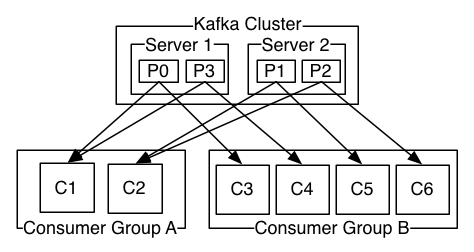
\includegraphics[width=0.42\textwidth]{consumer_groups.png}
    \caption{Consumer group trong Kafka.}
\end{wrapfigure}

Nhờ có group, Kafka đạt được lợi thế của cả cơ chế fan-out (nhiều loại group
consumer) và cơ chế load balancing (nhiều consumer để tăng tốc xử lý).

\subsubsection{Cluster Broker}

Trong Kafka, broker không phải là một máy riêng lẻ mà gồm nhiều máy khác nhau,
để phục vụ tính năng replication. Ngoài ra, Kafka còn dùng ZooKeeper để chứa cài
đặt broker. Toàn bộ các máy hợp lại thành một cụm broker.

\subsection{Phân mảnh và Nhân bản}

\subsubsection{Phân mảnh: cấu trúc log}

Trong Kafka, một topic được \emph{phân mảnh} thành các partition như sau:

\begin{figure}[H]
    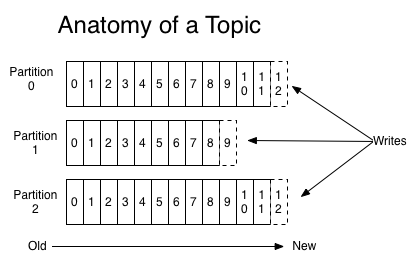
\includegraphics[scale=0.5]{log_anatomy.png}
    \centering
    \caption{Cấu trúc topic trong Kafka \cite{kafka_intro}.}
    \label{log_anatomy}
\end{figure}

Các partition này có cấu trúc log. Từ "log" ở đây hiểu theo nghĩa "một bản ghi
chỉ thêm vào đuôi", thể hiện cách dữ liệu được ghi. Các file log này chính là
cấu trúc dữ liệu cốt lõi của Kafka, là một trong hai yếu tố giúp Kafka có tốc độ
cao (sẽ nói ở phần sau).

Khi producer đưa một record vào topic, record đó sẽ được thêm vào đuôi một
partition, và được gán một số gọi là offset. Trong mỗi partition, số này tăng
dần theo các record được thêm vào, từ đó có thể thấy trong mỗi partition, các
record được sắp xếp theo thứ tự offset từ thấp đến cao, như trong hình
\ref{log_anatomy}.

Do việc ghi tuần tự vào đuôi mỗi log, việc đọc cũng trở nên dễ dàng. Consumer
chỉ cần nhớ offset gần nhất đã đọc, và đọc tuần tự tiếp từ đó, hoặc thậm chí có
thể trỏ offset về sâu nữa để xử lí dữ liệu cũ nếu cần.

Có một số lí do mà Kafka chia topic ra thành các partition:

\begin{itemize}
    \item Scale out: Nếu topic quá lớn, chỉ cần thêm máy broker và thêm
    partition.
    \item Tăng tốc xử lí: Một số trường hợp cần xử lí dữ liệu theo đúng trình tự
    thời gian, do đó chỉ được một consumer xử lí. Nếu không có partition, một
    consumer đó phải xử lí cả một topic. Vì có partition nên có thể dùng nhiều
    (nhưng vẫn không nhiều như load balacing) consumer, mỗi consumer xử lí một
    partition.
    \item Đánh đổi hợp lí giữa tốc độ và khả năng đảm bảo thứ tự: Với nhiều ứng
    dụng, thứ tự thông điệp rất quan trọng. Cách truyền thống là đảm bảo chỉ một
    consumer xử lí toàn bộ topic. Tuy nhiên Kafka chia topic ra các partition,
    và giao mỗi partition cho một consumer, do đó Kafka có thể tăng tốc độ xử lí
    (dĩ nhiên hệ thống sử dụng cũng cần được thiết kế phù hợp).
\end{itemize}

\subsubsection{Nhân bản: master-slave}

Mỗi partition có thể được nhân bản ra và lưu ở nhiều máy broker. Với mỗi
partition, có một máy broker được chọn làm master, và một số máy khác làm slave.
Các thao tác trên dữ liệu đều được thực hiện ở master, và cập nhật được lan
truyền sang các máy slave. Nếu master bị lỗi, ZooKeeper sẽ cử một slave lên làm
master.

Có hai lí do mà Kafka cần nhân bản partition:

\begin{itemize}
    \item Sao lưu
    \item Tăng tốc đọc: consumer có thể đọc từ nhiều máy broker (có từ Kafka
    2.4)
\end{itemize}

\subsection{Nhập/xuất hiệu năng cao}

Có hai lí do chính cho tốc độ cao của Kafka, và đều liên quan đến IO:

\subsubsection{Đọc ghi tuần tự}

Thông thường, ổ cứng được coi là quá chậm, phần vì lí do công nghệ ổ cứng, phần
vì người dùng có mẫu truy cập ngẫu nhiên. Theo bài test của Kafka, ổ cứng cơ
truyền thống nếu chạy RAID và ghi tuần tự có thể có băng thông 600 MB/s, tuy
nhiên cùng hệ thống ấy nếu ghi ngẫu nhiên thì chỉ được 1/6000 tốc độ ghi tuần
tự.

Do sử dụng cấu trúc log, việc ghi chỉ gồm ghi tuần tự vào cuối file (append),
việc đọc cũng tuần tự theo thứ tự offset (do ghi tuần tự nên đọc theo offset
cũng tuần tự), tốc độ đọc-ghi của Kafka rất nhanh. Kết hợp thêm ghi theo lô ở
phía producer và prefetch của hệ điều hành, Kafka có thể có thông lượng rất cao
mà không nhất thiết phải đầu tư vào SSD đắt tiền.

\subsubsection{Zero copy}

Thông thường, để gửi file qua socket, hệ điều hành cần làm lần lượt:

\begin{itemize}
    \item Đọc từ đĩa vào \emph{kernel} pagecache
    \item Đọc từ \emph{kernel} pagecache vào \emph{user-space} buffer
    \item Đọc từ \emph{user-space} buffer vào \emph{kernel} socket buffer
    \item Đọc từ \emph{kernel} socket buffer vào buffer card mạng
\end{itemize}

Với 4 lần copy và 2 lệnh hệ thống, cách này rất mất thời gian. Tuy nhiên, các hệ
điều hành hiện đại đều có cơ chế zero copy để copy trực tiếp vào buffer card
mạng, và Kafka tận dụng cơ chế này.

\subsection{Producer và Consumer}

\subsubsection{Producer}

Producer có thể chọn partition để ghi, và có thể gửi lệnh ghi theo lô để giảm
overhead.

\subsubsection{Consumer}

Giống với đa số các MOM khác, consumer lấy dữ liệu từ broker chứ không phải
broker "đẩy" dữ liệu xuống consumer.

\subsection{Ứng dụng}

Ứng dụng quan trọng nhất của Kafka chính là làm một hệ thống MOM.  Trong vai trò
này, Kafka đã được sử dụng thành công trong các hệ thống lớn, yêu cầu tốc độ
thời gian thực. Cụ thể hơn, có hai ca sử dụng phổ biến:

\begin{itemize}
    \item Event sourcing: Là một mô hình thiết kế. Trong mô hình này, các thay
    đổi trạng thái của dữ liệu được ghi lại và được gửi đến các hệ thống khác
    thông qua MOM. Với chuỗi các thay đổi này, bên nhận có thể "replay" và đạt
    được trạng thái dữ liệu của bên gửi.
    \item Analytic pipeline:
\end{itemize}

Ngoài ra, với hệ thống lưu trữ được phân mảnh và nhân bản, Kafka có thể đóng vai
trò làm một cơ sở dữ liệu.

Điểm khác biệt của Kafka và một số hệ thống đối thủ như ActiveMQ là mức độ hỗ
trợ cho xử lí dữ liệu dạng luồng (stream data). Dữ liệu dạng luồng coi dữ liệu
là một luồng đến và đi liên tục. Đây là quan điểm khác với quan điểm khác với ý
tưởng của xử lí dữ liệu theo lô (batch data), do để tạo được "lô" thì dữ liệu
phải có một cách phân nhóm hữu ích (ví dụ, nhóm dữ liệu theo năm). Với dữ liệu
dạng luồng, ngưòi ta chấp nhận rằng dữ liệu không thể được "gom" lại như thế
(hoặc chỉ "gom" một số điểm dữ liệu gần nhau). Từ đó, hệ thống dữ liệu luồng có
thể đạng được tốc độ xử lí gần với thời gian thực (do khối dữ liệu dùng để xử lí
nhỏ).

Các hệ thống MOM mới đều hỗ trợ phần nào các thao tác aggregator và join trong
xử lí dữ liệu dạng luồng, nhưng với các bài toán phức tạp hơn thì vẫn cần những
hệ thống xử lí luồng ở ngoài như Storm, Spark, ... Hiện tại chỉ Kafka mới có hệ
thống xử lí luồng riêng là Kafka Stream.

Tuy nhiên, các hệ thống MOM cổ điển hơn như ActiveMQ hay RabbitMQ, và các hệ
thống không broker (cho đến đây, các MOM được bàn đến đều có broker) như ZeroMQ
vẫn có chỗ đứng riêng. Một số nhược điểm của Kafka có thể kể đến là quá cồng
kềnh với một hệ thống nhỏ, đồng thời không hỗ trợ những thao tác phức tạp trên
dữ liệu như giao dịch (do đã đánh đổi cách lưu trữ dữ liệu phức tạp với hiệu
năng cao).

\section{Demo Kafka}

\subsection{Bài toán: Crawler}

Cho đường link một bài báo trên VnExpress hoặc Zing. Crawl dữ liệu (tiêu đề,
thân bài, ...) bài báo đó và các bài báo liên quan về.

\subsection{Lời giải}

Có một producer để nhận link bài báo từ người dùng, 2 consumer ứng với hai trang
báo để crawl dữ liệu. Có hai topic tương ứng với hai báo.

Khi producer nhận được link bài báo, nó kiểm tra xem bài báo là của báo nào, rồi
gửi vào topic tương ứng, đến consumer và crawler tương ứng. Dữ liệu crawl được
sẽ lưu lại ở dạng JSON và lưu ở thư mục gọi producer.

Chú ý, do Kafka tối ưu cho việc trao đổi thông tin một chiều/bất đồng bộ, do đó
không thế trả ngay dữ liệu crawl về như RMI hay các phương pháp
request-response. Thông thường nếu muốn tương tác hai chiêu, cần thêm một topic
nữa, và hai bên đổi vai trò producer-consumer cho nhau. Việc dựng thêm một topic
để trả về tận tay producer là rất khiên cưỡng, do producer rất nhỏ và chỉ gửi
thông tin một lần. Vì vậy, code demo không dùng cách này.

\emergencystretch=1em
\printbibliography[title={Tài liệu tham khảo}]

\end{document}
